\documentclass[11pt]{amsart}
\usepackage{geometry}                % See geometry.pdf to learn the layout options. There are lots.
\geometry{letterpaper}                   % ... or a4paper or a5paper or ... 
%\geometry{landscape}                % Activate for for rotated page geometry
%\usepackage[parfill]{parskip}    % Activate to begin paragraphs with an empty line rather than an indent
\usepackage{graphicx}
\usepackage{amssymb}
\usepackage{epstopdf}
\DeclareGraphicsRule{.tif}{png}{.png}{`convert #1 `dirname #1`/`basename #1 .tif`.png}

\title{Exploratory Data Analysis for Machine Learning: Honors Project}
\author{Jackson Walters}
\date{}                                           % Activate to display a given date or no date

\begin{document}
\maketitle
%\section{}
%\subsection{}

This project is for the Exploratory Data Analysis for Machine Learning certification from IBM via Coursera. The long-term goal is to create a t-SNE plot to observe clustering of mental health disorders based on symptom data, as in the linked paper\footnote{https://www.ncbi.nlm.nih.gov/pmc/articles/PMC6783390/}. I would like to include additional data based on life factors such as income, housing status, and insurance status. The idea is that if someone has no income, is unhoused, and uninsured then they would be much more likely to be classified as having a mental illness. I want to go beyond correlation, and see clustering. \\

For now, I implemented code from here \footnote{https://medium.com/@violante.andre/an-introduction-to-t-sne-with-python-example-47e6ae7dc58f}, and removed the SAS connection and written it in pure Python with sklearn. I did both PCA and t-SNE on the MNIST data, and plots are shown below. \\

All code is publicly available on GitHub \footnote{https://github.com/jacksonwalters/tsne-examples}

\begin{figure}[h]
\caption{t-SNE plot of MNIST handwritten digits data}
\centering
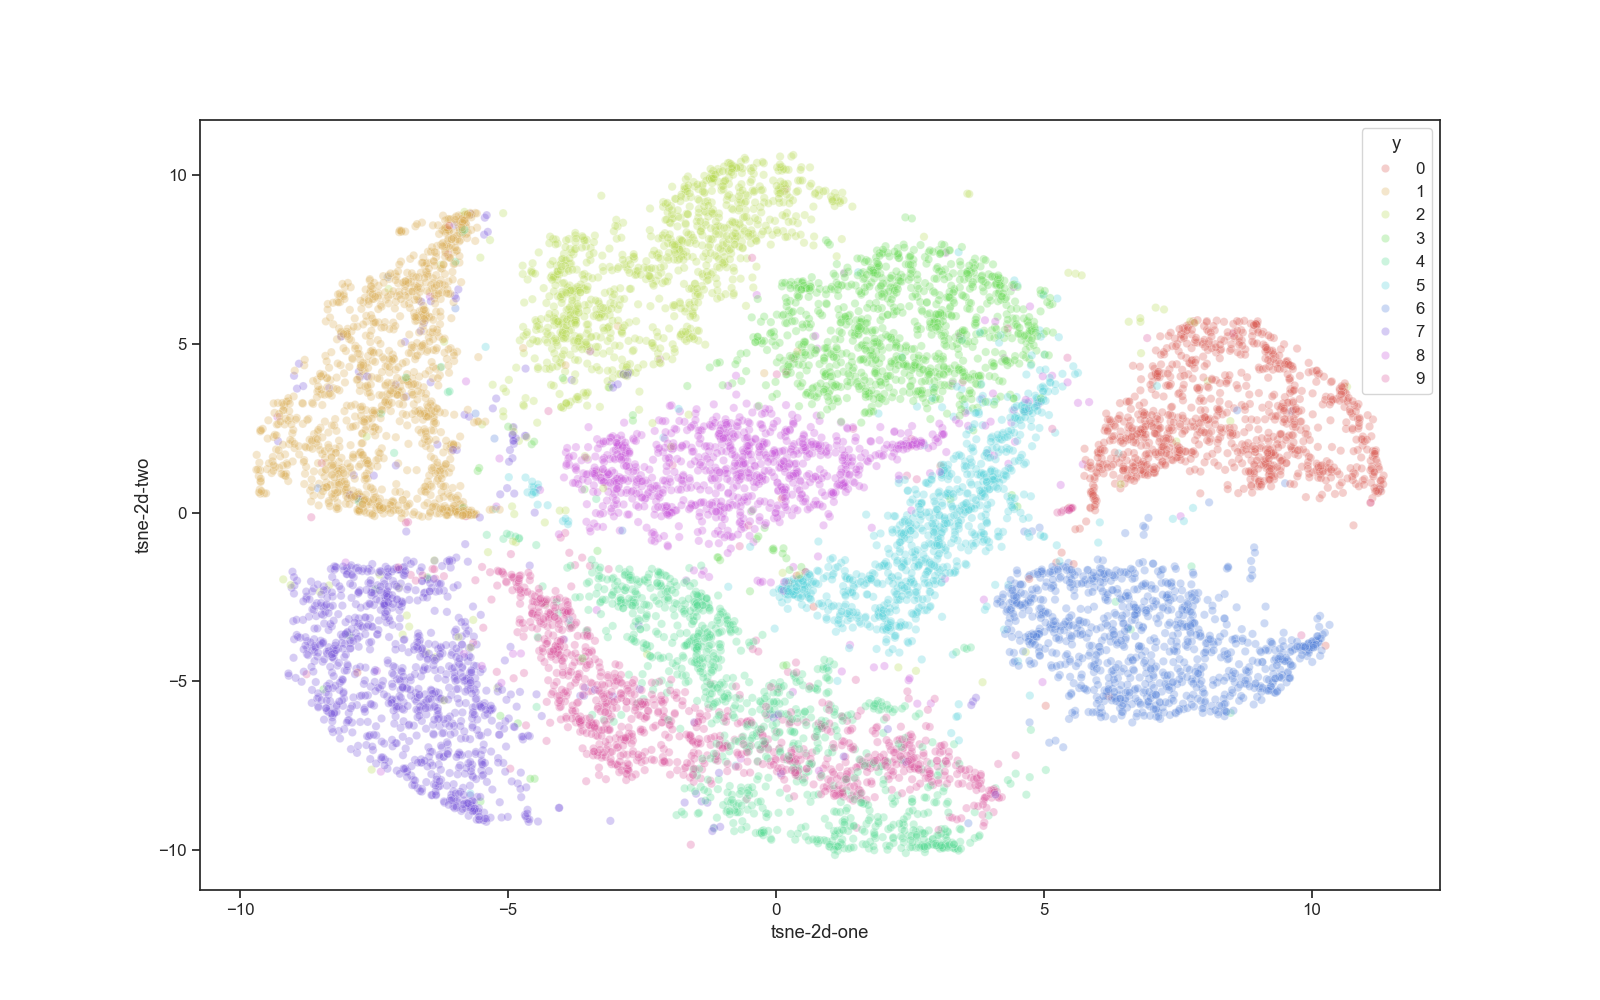
\includegraphics[width=0.5\textwidth]{t-SNE_plot_MNIST}
\end{figure}


\end{document}  